\section{Theorie}
\label{sec:Theorie}

Das menschliche Gehör ist in der Lage im Frequenzbereich von circa $\qty{16}{Hz}$ bis circa $\qty{20}{kHz}$ zu hören.
Im Bereich von $\qty{20}{kHz}$ bis $\qty{1}{GHz}$ wird von \textit{Ultraschall} gesprochen und bei Frequenzen darüber von \textit{Hyperschall}.
Unter der Hörschwelle wird von \textit{Infraschall} gesprochen.


\subsection{Grundlagen zu Ultraschall}

Die Ultraschallwellen breiten sich longitudinal aus.
Dabei sind die Amplituden die Druckschwankungen. 
Die Erzeugung von Ultraschall ist über verschiedene Wege möglich.
Ein Weg ist die Anwendung des reziproken \textit{piezo-elektrischen Effektes}.
Dafür wird ein piezoelektrischer Kristall in ein elektrisches Wechselfeld gegeben, sodass dieser zu Schwingungen angeregt wird.
Bei Schwingungen strahlt dieser dann Ultraschallwellen ab.
Wird die Anregungsfrequenz so gewählt, dass die Eigenfrequenz des Kristalls getroffen wird, entsteht der Resonanzfall.
Dabei können große Amplituden und Schallenergiedichten erzeugt werden.
Der Kristall, meistens ein Quarz, kann auch als Empfänger genutzt werden.

Da es sich um eine Welle handelt, kann diese durch die Wellenfunktion
\begin{equation}
    p(x, t) = p_0 + v_0 Z \cos (\omega t - k x)
\end{equation}
beschrieben werden. Dabei ist $Z = c \cdot \rho$ die akustische Impedanz, die durch die Dichte $\rho$
und der ebenfalls materialabhängigen Schallgeschwindigkeit $c$ gegeben ist.
Die materialabhängigen Schallgeschwindigkeit lässt sich durch die Gleichung
\begin{equation} \label{eq:clong}
    c_M = \sqrt{\frac{1}{\kappa \cdot \rho}}
\end{equation}
gegeben ist. $\kappa$ ist die Kompressibilität des Stoffes.
Da bei Festkörpern die Schallausbreitung durch die Schubspannungen nicht vollständig longitudinal sind, muss die \autoref{eq:clong} zu
\begin{equation}
    c_M ' = \sqrt{\frac{E}{\rho}}
\end{equation}
mit dem Elastizitätsmodul $E$ abgeändert werden.
In Festkörpern geht ein Teil der Energie durch Absorption verloren.
Die Intensität fällt dann exponentiell durch die Gleichung
\begin{equation}
    I(x) = I_0 \cdot e^{\alpha x}
\end{equation}
ab. Dabei ist $\alpha$ mit $\alpha < 0$ der Absorptionskoeffizient.
Dieser ist beispielsweise für Luft sehr hoch, weshalb in der Medizin ein Kontaktmittel bei Ultraschalluntersuchungen verwendet wird. \\

Bei Kontakt einer Schallwelle mit einem Medium wird ein Teil reflektiert und ein anderer tritt ein.
Der transmittierte Anteil wird durch
\begin{equation}
    T = 1 - R
\end{equation}
mit dem Reflexionskoeffizienten
\begin{equation}
    R = \left( \frac{Z_1 - Z_2}{Z_1 + Z_2} \right)^2.
\end{equation}

\subsection{Messverfahren mit Ultraschall}

Grundlegend gibt es im Bereich der Ultraschalltechnik zwei verschiedene Messmethoden in der Medizin.
Eins davon ist das \enquote{Durchschallungsverfahren}, dieses ist schematisch in \autoref{fig:Zeichnung1} dargestellt.
Dabei wird mit einer Ultraschallsonde ein kurzer Schallimpuls ausgesendet und am anderen Ende der Probe empfangen.
Es ist also nur möglich eine abgeschwächte Intensität zu messen, nicht jedoch die Fehlstelle der Probe zu ermitteln. 

Das andere Verfahren ist das \enquote{Impuls-Echo-Verfahren}, welches in \autoref{fig:Zeichnung2} dargestellt ist.
Dabei wird der Sender der Ultraschallwellen auch als Empfänger genutzt.
Das wird durch die Messung der Reflexion des Ultraschallpulses realisiert.
Ist die Schallgeschwindigkeit bekannt, kann auch die Fehlstelle durch die Gleichung
\begin{equation}
    s = \frac{1}{2} \, c \, t
\end{equation}
angegeben werden. Dabei ist t die Zeit, die der Puls ab Absenden bis zur Rückkehr zur Sonde braucht.
Die Ergebnisse können in sogenannten A-Scan's, B-Scan's oder TM-Scan's dargestellt werden.
\begin{figure}
    \centering
    \begin{subfigure}{0.49\columnwidth}
        \centering
        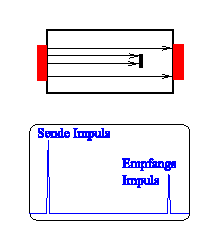
\includegraphics[width=\textwidth]{pictures/Zeichnung1.pdf}
        \caption{Das Impuls-Echo-Verfahren.}
        \label{fig:Zeichnung1}
    \end{subfigure}
    \hfill
    \begin{subfigure}{0.49\columnwidth}
        \centering
        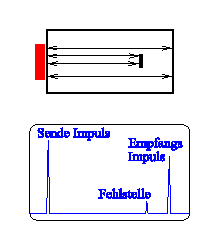
\includegraphics[width=\textwidth]{pictures/Zeichnung2.pdf}
        \caption{Das Durchschallungsverfahren.}
        \label{fig:Zeichnung2}
    \end{subfigure}
    \caption{Die beiden Ultraschallmessmethoden. \cite{us1}}
    \label{fig:verfahren}
\end{figure}